\documentclass[../mathNotesPreamble]{subfiles}

\providecommand{\relscalefact}{1.4}
\begin{document}
\relscale{\relscalefact}
  \section{2.5: Interpreting Graphs}

  {\noindent\Large\textbf{Appropriate Graphs:}}

  \noindent The type of data determines the type of graph you should use
  \begin{center}
    \begin{tabular}{@{}l@{\hspace*{15  mm}}l@{}}\toprule
      \textbf{Numerical Data}& \textbf{Categorical Data}\\\midrule
      Dot plot& Pie chart\\
      Histogram& Bar graph\\
      Stem-and-leaf plot& \\\bottomrule
    \end{tabular}
  \end{center}
  \vspace*{\stretch{1}}

  {\noindent\Large\textbf{Appropriate Measures:}}

  \noindent The type of data determines how the distribution of data should be described
  \begin{center}
    \begin{tabular}{@{}l@{\hspace*{15  mm}}l@{}}\toprule
      \textbf{Numerical Data}& \textbf{Categorical Data}\\\midrule
      Shape& Mode\\
      Center & ---\\
      Spread& Variability\\\bottomrule
    \end{tabular}
  \end{center}
  \vspace*{\stretch{1}}

  {\noindent\Large\textbf{Misleading Graphs:} \hfill\href[pdfnewwindow]{https://xkcd.com/2023/}{\textcolor{blue}{\underline{xkcd.com/2023}}}}

  \noindent\textbullet\ Inappropriate scaling (starting at a nonzero value)
  \begin{center}
    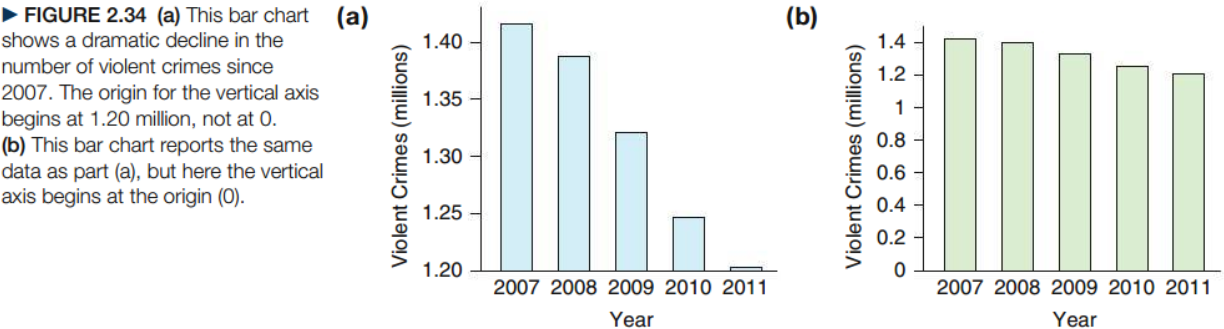
\includegraphics[width=0.95\linewidth]{images/math211_figure_2p34}
  \end{center}
  \pagebreak
  \noindent\textbullet\ Icons of different sizes instead of bars of proportionate heights:
  \begin{center}
    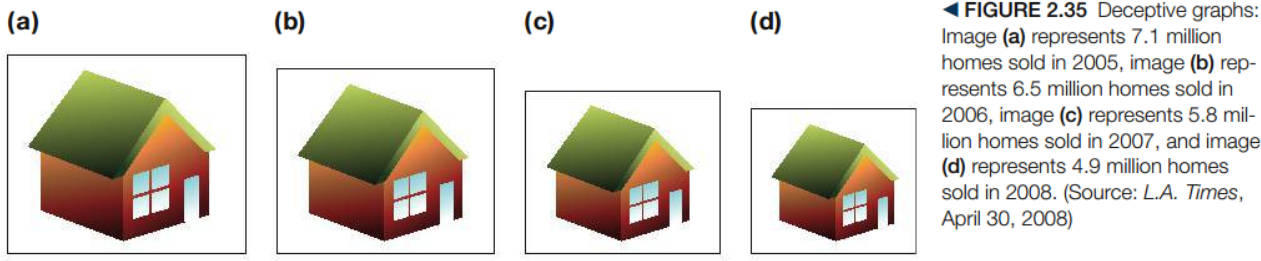
\includegraphics[width=0.95\linewidth]{images/math211_figure_2p35}
    \vspace*{\stretch{1}}

    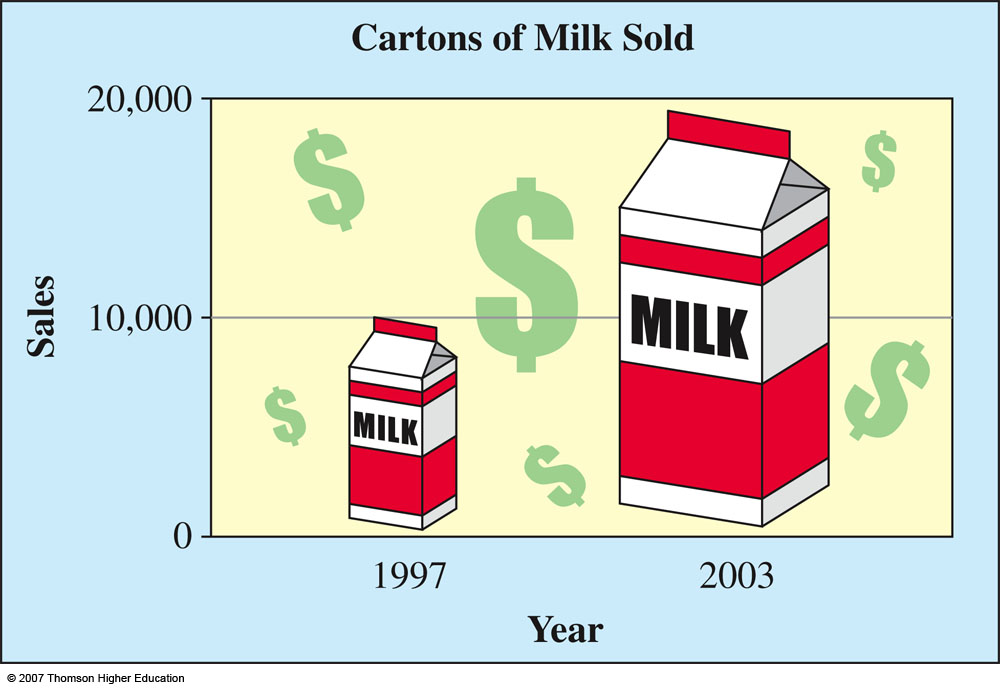
\includegraphics[width=0.65\linewidth]{images/math211_milk_icon}
  \end{center}
  \vspace*{\stretch{1}}
  \pagebreak

  \noindent\textbullet\ Avoid the use of 3D graphs:
  \begin{center}
    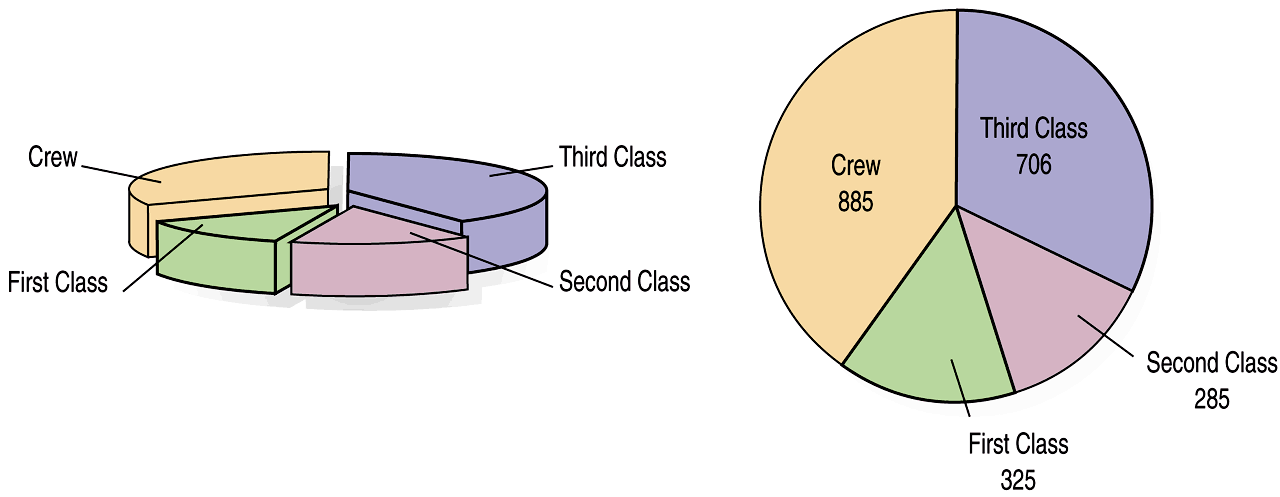
\includegraphics[width=0.9\linewidth]{images/math211_3d_pie_chart}
    \vspace*{\stretch{1}}

    \hspace*{\stretch{1}}
    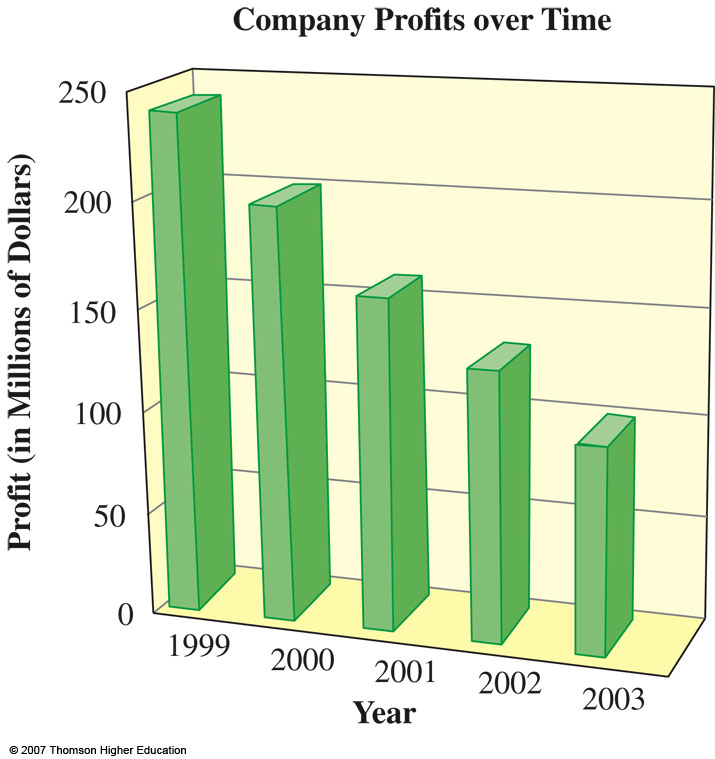
\includegraphics[width=0.35\linewidth]{images/math211_3d_bar_chart}
    \hspace*{\stretch{1}}
    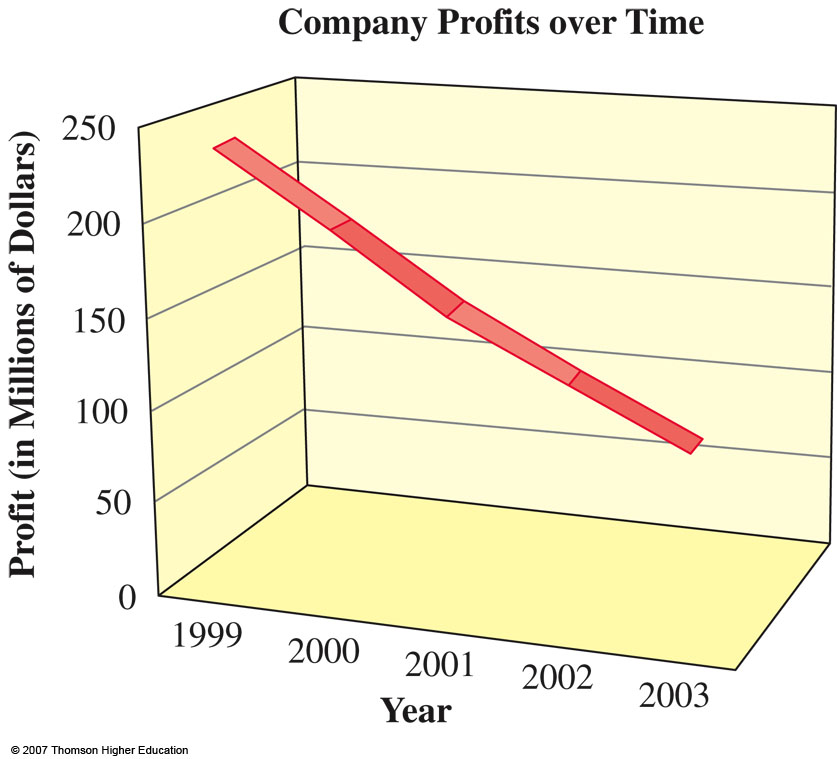
\includegraphics[width=0.35\linewidth]{images/math211_3d_line_chart}
    \hspace*{\stretch{1}}
  \end{center}
  \vspace*{\stretch{1}}

  \pagebreak
\end{document}
